% Metódy inžinierskej práce

\documentclass[10pt,onecolumn,twoside,english,a4paper]{article}

% \usepackage[slovak]{babel}
%\usepackage[T1]{fontenc}
\usepackage{graphicx}
\graphicspath{ {./} }
\usepackage[IL2]{fontenc} % lepšia sadzba písmena Ľ než v T1
\usepackage[utf8]{inputenc}
\usepackage{graphicx}
\usepackage{url} % príkaz \url na formátovanie URL
\usepackage{hyperref} % odkazy v texte budú aktívne (pri niektorých triedach dokumentov spôsobuje posun textu)
\usepackage{subfig} 
\usepackage{cite}
\usepackage{amsmath}
\usepackage{wrapfig}
% \usepackage{}
%\usepackage{times}
\usepackage{tikz}
\usepackage{blindtext}
% \usepackage[parfill]{parskip}
\usetikzlibrary{automata, positioning, arrows}
\usetikzlibrary{arrows.meta}
\usepackage{pgfplots} 
% \usepackage{indentfirst}
\pagestyle{headings}
% \setlength{\parskip}{0pt}

\pgfplotsset{compat=1.18}
\usepgfplotslibrary{external}
\tikzexternalize

\title{Overview and Analysis of GPU Acceleration for Regular Expressions
\thanks{Semestjrálny projekt v predmete Metódy inžinierskej práce, ak. rok 2023/24, vedenie: MSc. Mirwais Ahmadzai}} % meno a priezvisko vyučujúceho na cvičeniach

\author{Roman Gajdoš\\[2pt]
	{\small Slovak University of Technology in Bratislava}\\
	{\small Faculty of Informatics and Information Technologies}\\
	{\small \texttt{xgajdosr@stuba.sk}}
	}

\date{\small 25. september 2023} % upravte



\begin{document}

\maketitle

\begin{abstract}
  Pattern matching is essential across numerous domains and regular expressions are a fundamental component. They are used in various applications, including database queries, network security, bioinformatics and more. It is crucial to ensure efficient use of memory and speed, particularly when handling vast datasets or time-sensitive tasks.
  Conventional processors face limitations in their ability to execute parallel tasks. However, Graphics Processing Units (GPUs) have become prevalent in many computing systems and offer a promising solution with extensive parallelism, computational capacity, and high memory bandwidth.

  This paper provides a comprehensive overview of GPU-accelerated regular expressions, including comparative analysis and reference to previous studies. Our investigation into the acceleration of regular expressions illustrates the potential of the GPU as a practical platform for pre-processing, which outperforms other platforms in terms of speed, but sometimes operates with a lower throughput. Moreover, we demonstrate variations in the performance of finite automata representations and their effect, explaining that the NFA representation is more efficient in terms of memory, whereas the DFA representation is more rapid. We also note the need for further research in this area. There has been minimal recent exploration, specifically regarding the potential combination of different accelerator platforms with GPUs for regular expression acceleration or examination of OpenCL in comparison to CUDA is yet to be undertaken, and would benefit from investigation.

\end{abstract}

\section{Introduction} \label{Introduction}
Pattern matching is widely used in a variety of different domains. Regular expressions have become a prevalent tool for text processing and sanitation due to their flexibility, conciseness, and vast support in most programming languages\cite{Chapman:Usage}. They appear in approximately a third of open-source projects\cite{Davis:Re-use}. They are employed in technical fields, ranging from database querying\cite{István:databases-regex}, texts editors\footnote{\url{https://neovim.io/doc/user/change.html\#\%3Asubstitute}}, web scraping \cite{Gunawan2019/03} to network security, such as deep packet inspection \cite{becchi2008workload}, and bioinformatics \cite{huang2008gpu}, among others.

Regular expressions are implemented using finite automata, in either deterministic (DFA) or non-deterministic (NFA) form, each with their respective advantages and drawbacks. Each of them has their own advantages and disadvantages \cite{Becchi:regex_large_dataset,Nourian:DemystifyingFSA,Zu:GPU-NFA}.

In many applications, regular expressions are applied to large amounts of input data, or require a fast response, or both. It stands to reason that efficiency in both memory and speed is the key to optimal use\cite{Xia:FSA-scaling}.
Here, the question is how to achieve the greatest possible efficiency for a given problem that is addressed by the regular expressions.

The processor's capacity to execute multiple expressions simultaneously is notably restricted, even in the current era of multicore processors\cite{Lee:myths}. However, its frequency and cache memory speed prove excellent for handling small datasets. For tasks that require more extensive parallelism, FPGAs (Field-Programmable Gate Arrays) or ASICs (Application-Specific Integrated Circuits) have been used. The problem is that they are slow to configure\cite{XU:regex_alg_slow} and inflexible to change \cite{fuchs2019accelerator,Liu:Asynchronous}.

In recent years, GPUs with their extensive parallelism, computational capabilities, and high memory bandwidth have become prevalent in numerous computing system. They have scaled at a faster rate than CPUs, providing significant computing power\cite{sun2019summarizing,Liu:Asynchronous}. APIs were created to allow General Purpose Graphics Processing Units (GPGPU) to accelerate processing in supported applications, replacing shading languages and simplifying their use for programmers. Two popular APIs are Compute Unified Device Architecture (CUDA) and Open Computing Language (OpenCL)\cite{Fang:Comparison-cuda-opencl}.

In this paper, we investigate a variety of GPU-based regular expression execution methods and conduct a comparative analysis of their strengths and weaknesses. Our research begins with a thorough examination of regular expressions in~\ref{Background}. This is followed by a comparison of their representations of finite state automata forms in \ref{Finite Automata}. We then move into parallel computing platforms, such as CUDA and OpenCL in \ref{Parallel computing platforms}.

By combining these findings, our investigation aims to provide a comprehensive overview of GPU-accelerated regular expressions, utilizing previous studies to provide an in-depth comparative analysis in section ~\ref{Related work} and \ref{Analysis}. Result from this was evaluated in the \ref{Results} section. Finally, we conclude with a summary of our findings in section ~\ref{Conclusions}.

\section{Objective and methodology} \label{Objective}
At present, we are unaware of any comprehensive analysis of the available materials on the acceleration of regular expressions on GPU. We have therefore decided to review the available data to see if there are any conflicting statements or claims that have evolved over time or are no longer valid. The outcome ought to be an in-depth, up-to-date article showing when to use GPU regular expression acceleration, what its benefits are, and when other solutions are better.

In this research, we will compare data from papers on or relevant to this topic and look at how the results have changed over time. We will also look at the various methods of accelerating regular expressions on GPUs and compare their strengths and weaknesses.
We will maintain an unbiased perspective and present information in a clear and concise manner. Technical terminology will be firstly explained in separate section.


\section{Background} \label{Background}
A regular expression, or regex for short, represents a set of exactly matching strings of characters and special symbols. This set can be infinite. The string of characters is then matched against the pattern to see if it matches. Regular expressions can be constructed in several ways~\cite{wang2014techniques}. The most common is to use a formal language, such as the one in POSIX standard\footnote{\url{https://pubs.opengroup.org/onlinepubs/9699919799/basedefs/V1_chap09.html}}.
Basic syntax is described as follows: characters of alphabet are matched literally, special symbols are used to match a single/multiple character matches, optional character matches, alternation, any character, line start/end and the empty string. As described in table \ref{table:regex_special_symbols}.


% latex table of special symbols
\begin{table}[h!]
  \centering
  \begin{tabular}{ |c|c| }
    \hline
    \textbf{Symbols}        & \textbf{Meaning}                 \\
    \hline
    \texttt{.}              & Any character                    \\
    \hline
    \texttt{*}              & Zero or more matches             \\
    \hline
    \texttt{+}              & One or more matches              \\
    \hline
    \texttt{?}              & Zero or one match                \\
    \hline
    \texttt{|}              & Alternation                      \\
    \hline
    \texttt{-}              & Range                            \\
    \hline
    \texttt{\textbackslash} & Escape character                 \\
    \hline
    \texttt{\^{}}           & Line start                       \\
    \hline
    \texttt{\$}             & Line end                         \\
    \hline
    \texttt{:}              & Grouping                         \\
    \hline
    \texttt{[ ]}            & Start and end of character class \\
    \hline
    \texttt{( )}            & Start and end of group           \\
    \hline
    \texttt{\{ \}}          & Start and end of quantifier      \\
    \hline
  \end{tabular}
  \caption{Regular expression special symbols, author's own work }
  \label{table:regex_special_symbols}
\end{table}

\subsection{Finite Automata} \label{Finite Automata}
Regular expression matching is performed by using finite automata, a mathematical model of computation that abstracts computations into a finite number of states and transitions \cite{Becchi:regex_large_dataset}. A finite automaton comprises a directed graph in which each node symbolises a state while each edge reflects a state transition.
Two widely used representations of finite automata are deterministic finite automata (DFAs) and non-deterministic finite automata (NFAs). While NFAs and DFAs achieve the same outcome, there are some practical differences in terms of resource requirements and traversal behaviour \cite{Nourian:DemystifyingFSA}.
Although deterministic finite automata (DFAs) have a simpler transition system, their execution is serial and the size of transitions in DFAs may be significantly larger than their equivalent NFAs \cite{Liu:Asynchronous,Liu:WhyGPUSlowNFA}.

\begin{figure}[h!]
  \tikzset{
    ->, % makes the edges directed
    >=stealth', % makes the arrow heads bold
    node distance=3cm, % specifies the minimum distance between two nodes. Change if necessary.
    every state/.style={thick, fill=gray!10}, % sets the properties for each ’state’ node
    initial text=$ $, % sets the text that appears on the start arrow
  }
  \centering
  \scalebox{.7}[.7]{
    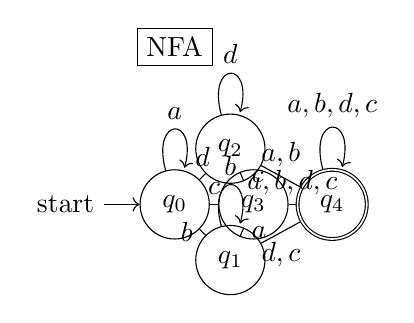
\begin{tikzpicture}
      \node[draw] at (0,2) {NFA};
      \node[state, initial] (q0) {$q_0$};
      \node[state, below right of=q0] (q1) {$q_1$};
      \node[state, above right of=q0] (q2) {$q_2$};
      \node[state, right of=q0] (q3) {$q_3$};
      \node[state, accepting, right of=q3] (q4) {$q_4$};
      \draw (q0) edge[loop above] node{$a$} (q0)
      (q0) edge[right,above] node{$c$} (q3)
      (q0) edge[left] node{$b$} (q1)
      (q0) edge[right, above] node{$d$} (q2)
      (q1) edge[loop above] node{$b$} (q1)
      (q1) edge[right] node{$a$} (q3)
      (q1) edge[below] node{$d,c$} (q4)
      (q2) edge[loop above] node{$d$} (q1)
      (q2) edge[right] node{$c$} (q3)
      (q2) edge[above ] node{$a,b$} (q4)
      (q3) edge[above] node{$a,b,d,c$} (q4)
      (q4) edge[loop above] node{$a,b,d,c$} (q4)
      ;
    \end{tikzpicture}
  }
  \scalebox{.7}[.7]{
    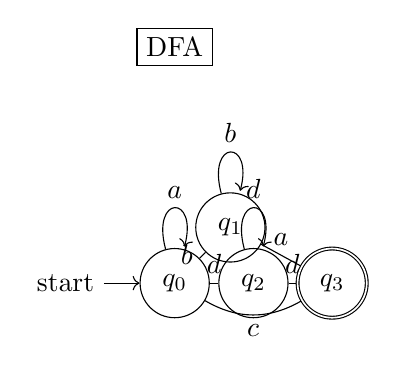
\begin{tikzpicture}
      \node[draw] at (0,3) {DFA};
      \node[state, initial] (q0) {$q_0$};
      \node[state, above right of=q0] (q1) {$q_1$};
      \node[state, right of=q0] (q2) {$q_2$};
      \node[state, accepting, right of=q2] (q3) {$q_3$};
      \draw (q0) edge[loop above] node{$a$} (q0)
      (q0) edge[bend right,below] node{$c$} (q3)
      (q0) edge[left] node{$b$} (q1)
      (q1) edge[loop above] node{$b$} (q1)
      (q2) edge[loop above] node{$d$} (q1)
      (q1) edge[above] node{$a$} (q3)
      (q0) edge[right, above] node{$d$} (q2)
      (q2) edge[right, above] node{$d$} (q3)
      ;
    \end{tikzpicture}
  }
  \caption{NFA and DFA for regular expression \texttt{a*(b+a|d*c)}, autor's own work}
  \label{fig:regex_FSA}
\end{figure}

\subsubsection{Automata processing} \label{Automata processing}
The regular expression's matching process is equivalent to a finite state machine traversal of the input stream.
The process of matching begins with the activation of the initial states. Symbols from the input stream are sequentially utilized by the finite automaton.The process concludes once all the symbols of the input stream are processed.The incoming symbol is matched with the active states, and if it falls within the matchset of an active state, the active state transforms into a matched state \cite{Liu:Asynchronous}.

We can guarantee worst-case performance by restricting the processing of each input character. Techniques to limit per-character processing involve enlarging the finite automaton. Therefore, the search space is determined by balancing the size of the automaton and the upper limit of per-character processing \cite{Nourian:DemystifyingFSA}.

The benefit of using NFA is its capability to construct an NFA consisting of states that are less than or equal to the number of characters in the pattern-set. This makes the representation compact. The primary deficiency of NFAs lies in their traversal, during which the number of active states can vary from iteration to iteration, as well as the amount of work performed\cite{Becchi:regex_large_dataset}.

\subsection{Graphics Processing Unit} \label{GPU}
The GPU, or Graphics Processing Unit, offers significantly higher instruction throughput and memory bandwidth than the CPU at a comparable price and power consumption.
While the CPU is optimized for rapid execution of a sequence of operations referred to as a "thread" and can execute dozens of these threads concurrently, the GPU is optimized for thousands of parallel executions (offsetting the slower single-thread performance for increased throughput).This variation in capabilities is a result of differing design objectives for the GPU and CPU.\footnote{From \url{https://docs.nvidia.com/cuda/cuda-c-programming-guide/index.html}}

All threads within a compute unit share a common instruction counter. Execution of a single compute unit occurs in lock-step, whereby each thread executes the same instruction when directed to do so. When control flow divergence occurs between threads within the same work group, divergent instructions are serialised,which can negatively impact performance.
Similarly, an unbalanced workload across threads in a work-group will result in idle threads, which reduces performance~\cite{yaneva2022gpuaccelerationFSA}.

The memory hierarchy of GPUs comprises: Global memory, a larger and slower form of memory accessible by all threads in any compute units. Constant memory, a read-only section of the global memory with a specific cache for faster memory access. Local memory, connected to compute units and shared among threads in a single unit and private memory, exclusively reserved for individual threads~\cite{yaneva2022gpuaccelerationFSA}.

\subsubsection{Parallel computing platforms} \label{Parallel computing platforms}
Due to the significant performance potential of GPUs, their  utilization has evolved from high-level shading languages to modern programming languages, reducing time and complexity involved in creating GPU-enabled applications~\cite{Asaduzzaman:Impact_CUDA_OpenCL}.
Two of the most popular APIs for GPU programming are CUDA\footnote{\url{https://developer.nvidia.com/cuda-toolkit}} (Compute Unified Device Architecture) and OpenCL\footnote{\url{https://www.khronos.org/opencl/}} (Open Computing Language). CUDA is a proprietary API developed by NVIDIA, while OpenCL is s an open royalty-free standard developed by the Khronos Group (an open, member-driven consortium, publishing and maintaining open standarts) \footnote{\url{https://www.khronos.org/}}.

OpenCL provides an efficient and portable way to access the power of different computing platforms. However, when comparing OpenCL to CUDA, there are sometimes performance differences. These differences are often attributed to the portability of OpenCL, which can lead to performance degradation. However, in a fair comparison, there is no inherent reason for OpenCL to perform worse than CUDA. Performance differences are primarily due to programmers and compilers behaviour\cite{Fang:Comparison-cuda-opencl}.

\section{Related Work} \label{Related work}
Research into the use of GPUs for regular expression matching started with the publications "\textit{Fast Exact String Matching on the GPU}"\cite{schatz2007fast} and "\textit{A GPU-based Multiple-pattern Matching Algorithm for Network Intrusion
  Detection Systems}"\cite{huang2008gpu}. Their pioneering studies introduced a string matching program and multiple-pattern matching algorithm designed to take advantage of GPU processing capabilities.
This work was soon followed by "\textit{Accelerating Regular Expression Matching Using Hierarchical Parallel Machines on GPU}"\cite{Lin:regex_gpu_parallel} and "\textit{GPU-based NFA Implementation for Memory Efficient High Speed Regular Expression Matching}"\cite{Zu:GPU-NFA}. These two studies provide solutions to the performance challenges linked to regular expression matching in the context of network intrusion detection and other network functions.

Afterwards, a large, comprehensive study entitled "\textit{GPU Acceleration of Regular Expression Matching for Large Datasets: Exploring the Implementation Space}"\cite{Becchi:regex_large_dataset} was published. The study examines regular expression matching on GPUs, focusing on practical-sized and complex datasets. It explores the advantages and limitations of different automata representations and various GPU implementation techniques.

In the paper "\textit{Demystifying Automata Processing: GPUs, FPGAs or Micron's AP?}"\cite{Nourian:DemystifyingFSA}, the authors compare the performance of GPUs, FPGAs, and Micron's Automata Processor (AP) for regular expression matching.

Later, studies were published dealing with speeding up the processing of finite state machines. Papers "\textit{Scaling Out Speculative Execution of Finite-State Machines with Parallel Merge}"\cite{Xia:FSA-scaling} based on "\textit{On-the-Fly Principled Speculation for FSM Parallelization}"\cite{zhao2015fly} introduce a speculative execution technique for finite state machines. "\textit{Why GPUs are Slow at Executing NFAs and How to Make them Faster}"\cite{Liu:WhyGPUSlowNFA} proposed and evaluated optimisations to improve the throughput of NFA processing on GPUs by addresing tackle suboptimal data movement and underutilisation.
"\textit{Asynchronous Automata Processing on GPUs}"\cite{Liu:Asynchronous} have developed a lightweight approach to increase the parallelism of automata processing on GPUs by asynchronously searching for patterns in the input stream in parallel.

\marginpar{GPU acceleration of finite state machine input execution:
  Improving scale and performance.
  nieco o CUDA/OPENCL}

\section{Analysis} \label{Analysis}
\subsection{GPU Acceleration of Regular Expression Matching for Large Datasets: Exploring the Implementation Space} \label{Becchi:regex_large_dataset_analysis}
This study\cite{Becchi:regex_large_dataset}, published in 2013, was the first to make relevant measurements using real-life data. The measurements were conducted using NFA design by \cite{cascarano2010infant}, along with their optimised NFA; and DFA design by \cite{becchi2007improved}, in uncompressed (U-DFA), compressed (C-DFA), and optimized (E-DFA) forms.

Their dataset used both real and synthetic pattern sets. The real patterns were taken from Snort's backdoor and spyware rules. The synthetic sets were generated using a tool described in \cite{becchi2008workload} and tokens from the backdoor rules.

Measurements were made on system consisting of Xeon E5620 CPU and an NVIDIA \marginpar{CUDA cores maybe} GTX 480 GPU\footnote{cuda cores}, using CentOS 5.5 and CUDA 4.
\subsubsection{Study findings}
The repetition of wildcards and large character sets can lead to a state explosion when converting an NFA to a DFA. On the chart \ref{dfas_size:becchi}, we can see size of DFAs in MB. In contrast, NFAs are consistently less than 1 MB in size. For synthetic datasets, the uncompressed DFA representation has 40-50 times the memory requirement of its compressed counterpart. At the time of writing, the Dotstar.2 datasets exceed the device memory capacity when uncompressed-DFA representation is utilized.
\begin{figure}[h!]
  \centering
  % \scalebox{.9}[.9]{
  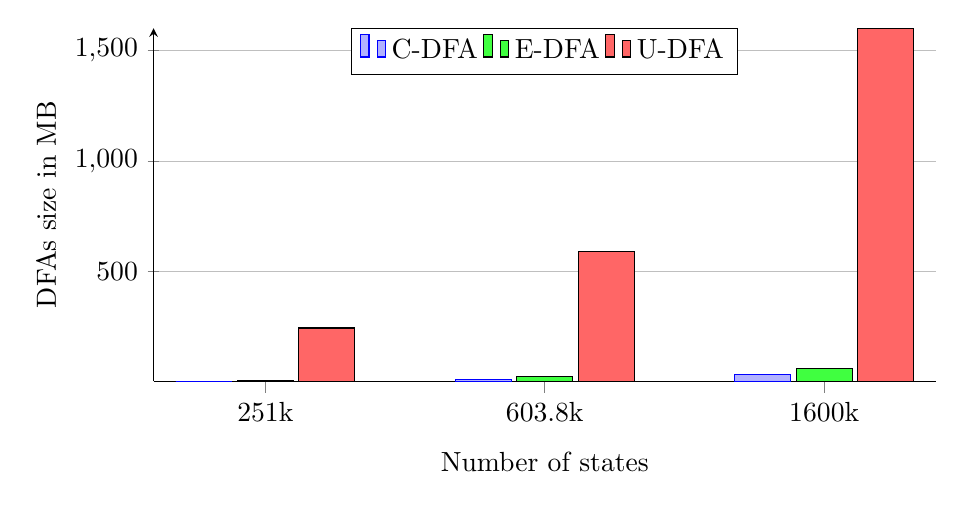
\begin{tikzpicture}
    \begin{axis}[
        ylabel=DFAs size in MB,
        xlabel=Number of states,
        enlargelimits={abs=0.4},
        legend style={at={(0.5,1)},
            anchor=north,legend columns=3},
        ybar,
        bar width=0.2, % Adjust the width as needed
        xtick=\empty, % Remove numbers on the x-axis
        width=0.95 \textwidth,
        height=0.5 \textwidth,
        extra x ticks={1, 2, 3}, % Add extra ticks at positions 1, 2, and 3
        extra x tick labels={251k, 603.8k, 1600k}, % Label the extra ticks
        % remove just frame, not ticks
        axis x line*=bottom,
        axis y line=left,
        ymajorgrids=true,
      ]
      \addplot
      coordinates {
          (1, 6.2)
          (2, 15.2)
          (3, 33.9)
        };
      \addplot[
        fill=green!75, % Set a custom color for this bar
      ]
      coordinates {
          (1, 10)
          (2, 26)
          (3, 63.4)
        };
      \addplot[
        fill=red!60, % Set a custom color for this bar
      ]
      coordinates {
          (1, 246)
          (2, 592)
          (3, 1600)
        };
      \legend{C-DFA, E-DFA, U-DFA}
    \end{axis}
  \end{tikzpicture}
  \caption{Scaling of DFAs size, author's own work, data from \cite{Becchi:regex_large_dataset}}
  \label{dfas_size:becchi}
\end{figure}

As shown in chart \ref{speed NFA/DFA:becchi}, the U-DFA is the optimal solution for all pattern-sets, when applicable. However, this solution has high memory requirements and cannot be applied to complex pattern-sets due to a lack of graphics card memory.
E-DFA offers a reasonable trade-off between U-DFA and C-DFA, resulting in a 3-5 times enhancement in speed compared to C-DFA at the expense of almost 1.5X more memory usage. Moreover, E-DFA performs better than NFA solutions on nearly all datasets.

\begin{figure}[h!]
  \centering
  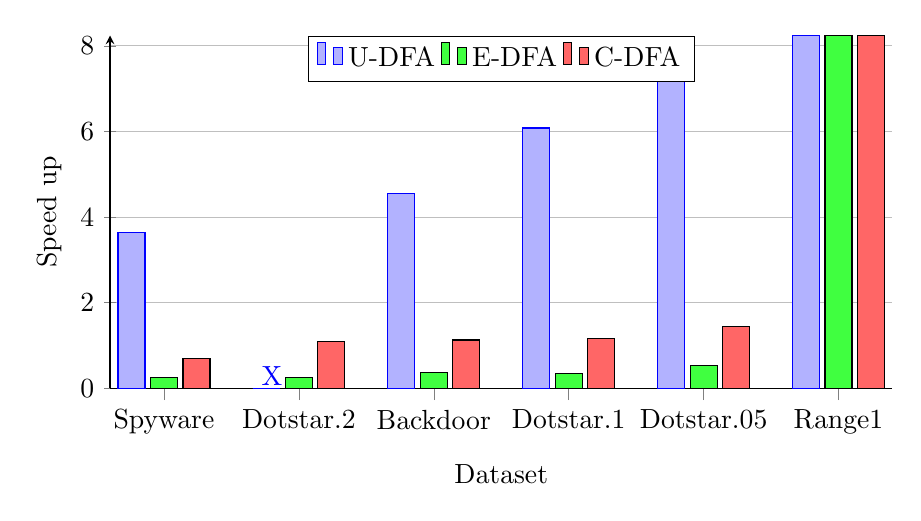
\begin{tikzpicture}
    \begin{axis}[
        ylabel=Speed up,
        xlabel=Dataset,
        enlargelimits={abs=0.4},
        legend style={at={(0.5,1)},
            anchor=north,legend columns=3},
        ybar,
        bar width=0.2, % Adjust the width as needed
        xtick=\empty, % Remove numbers on the x-axis
        width=0.95 \textwidth,
        height=0.5 \textwidth,
        extra x ticks={1, 2, 3, 4, 5, 6}, % Add extra ticks at positions 1, 2, and 3
        extra x tick labels={Spyware, Dotstar.2, Backdoor, Dotstar.1, Dotstar.05, Range1}, % Label the extra ticks
        % remove just frame, not ticks
        axis x line*=bottom,
        axis y line=left,
        ymajorgrids=true,
      ]
      \addplot
      coordinates {
          (1, 3.63)
          (2, 0)
          (3, 4.56)
          (4, 6.08)
          (5, 7.39)
          (6, 8.24)
        };
      \addplot[
        fill=green!75, % Set a custom color for this bar
      ]
      coordinates {
          (1, 0.25)
          (2, 0.26)
          (3, 0.37)
          (4, 0.34)
          (5, 0.53)
          (6, 8.24)
        };
      \addplot[
        fill=red!60, % Set a custom color for this bar
      ]
      coordinates {
          (1, 0.69)
          (2, 1.10)
          (3, 1.13)
          (4, 1.16)
          (5, 1.44)
          (6, 8.24)
        };
      \node[blue] at (axis cs:1.8,0.3) {X}; % Adjust the color
      \legend{U-DFA, E-DFA, C-DFA}
    \end{axis}
  \end{tikzpicture}
  \caption{Speedup of DFA's over NFA, author's own work, data from \cite{Becchi:regex_large_dataset}}
  \label{speed NFA/DFA:becchi}
\end{figure}

As shown in chart \ref{speedup:becchi}, both GPU implementations based on NFA and DFA algorithms outperformed their CPU equivalent.

\begin{figure}[h!]
  \centering
  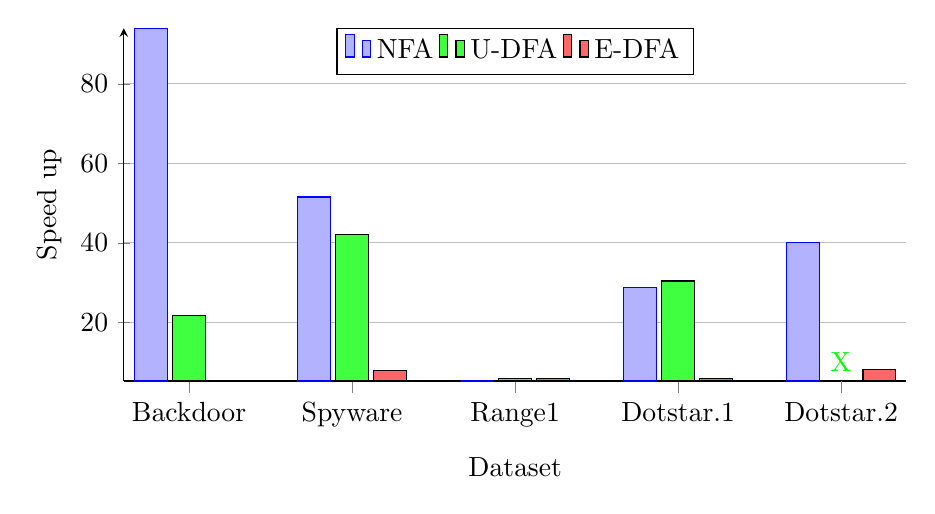
\begin{tikzpicture}
    \begin{axis}[
        ylabel=Speed up,
        xlabel=Dataset,
        enlargelimits={abs=0.4},
        legend style={at={(0.5,1)},
            anchor=north,legend columns=3},
        ybar,
        bar width=0.2, % Adjust the width as needed
        xtick=\empty, % Remove numbers on the x-axis
        width=0.95 \textwidth,
        height=0.5 \textwidth,
        extra x ticks={1, 2, 3, 4, 5}, % Add extra ticks at positions 1, 2, and 3
        extra x tick labels={Backdoor, Spyware, Range1, Dotstar.1, Dotstar.2}, % Label the extra ticks
        % remove just frame, not ticks
        axis x line*=bottom,
        axis y line=left,
        ymajorgrids=true,
      ]
      \addplot
      coordinates {
          (1, 94)
          (2, 51.55555556)
          (3, 5.244897959)
          (4, 28.88888889)
          (5, 40)
        };
      \addplot[
        fill=green!75, % Set a custom color for this bar
      ]
      coordinates {
          (1, 21.69620253)
          (2, 42.05)
          (3, 5.846153846)
          (4, 30.40384615)
          (5, nan)
        };
      \addplot[
        fill=red!60, % Set a custom color for this bar
      ]
      coordinates {
          (1, 5.392405063)
          (2, 7.95)
          (3, 5.846153846)
          (4, 5.807692308)
          (5, 8.21875)
        };
      \node[green] at (axis cs:5,10) {X}; % Adjust the color
      \legend{NFA, U-DFA, E-DFA}
    \end{axis}
  \end{tikzpicture}
  \caption{Speed up of GPU accelerated traversals over CPU, author's own work, data from \cite{Becchi:regex_large_dataset}}
  \label{speedup:becchi}
\end{figure}

\subsection{Demystifying Automata Processing: GPUs, FPGAs or Micron's AP?} \label{Nourian:DemystifyingFSA_analysis}
This 2017 study\cite{Nourian:DemystifyingFSA} investigated the acceleration of Finite State Automata on GPU, FPGA and Micron's AP. The automata model employed was NFA, and the algorithm used for its traversal engine was described in \cite{van2012designing}.

Their dataset consists of small NIDS, bioinformatics and synthetic pattern sets.
The measurements were performed on a system that consisted of a dual 6-core Intel Xeon CPU and an Nvidia Titan X GPU\footnote{cuda cores} (Maxwell architecture), using CentOS 6.4 and CUDA 7. The FPGA Xilinx XC6VLX130T was chosen as it fell in the same price range as the GPU (approximately \$1,200 at that time).

\subsubsection{Study findings}
The NFA format for GPU has a very small global memory utilisation, and even the largest dataset only occupies up to 133MB of global memory, which means we are able to fit any size dataset into a single GPU device, unlike FPGA and Micron's AP, which required more devices, as shown in the graph \ref{devices:DemystifyingFSA}. However, the GPU records the lowest throughput data, with a 20 times lower throughput on smaller datasets up to 1000 times lower on the largest datasets.
% chart of devices used with dataset 
% deep64char	deep256char	shallow64char	shallow256char
% GPU	1	1	1	1
% FPGA	8	8	7	8
% Micron's AP	3	3	5	3
\begin{figure}[h!]
  \centering
  % \scalebox{.9}[.9]{
  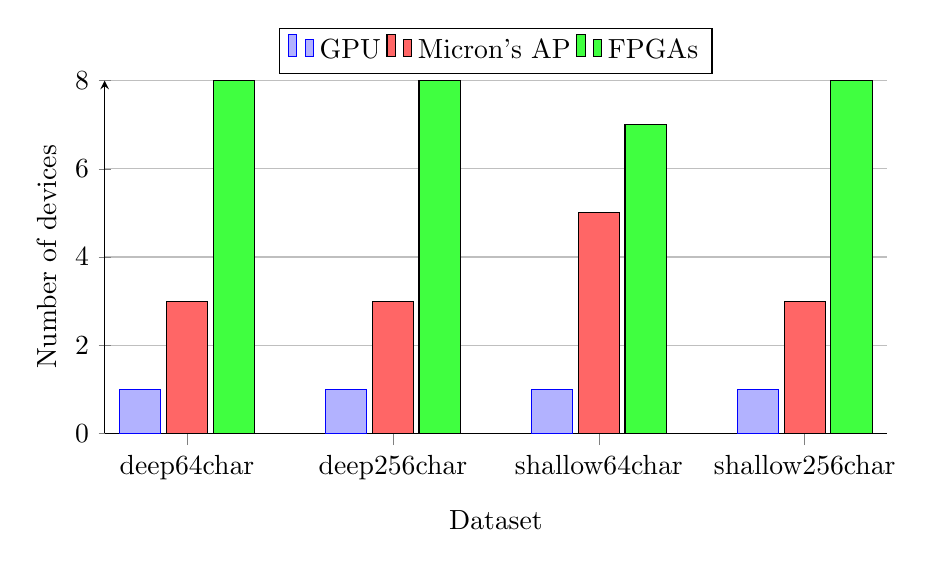
\begin{tikzpicture}
    \begin{axis}[
        ylabel=Number of devices,
        xlabel=Dataset,
        enlargelimits={abs=0.4},
        legend style={at={(0.5,1.15)},
            anchor=north,legend columns=3},
        ybar,
        bar width=0.2, % Adjust the width as needed
        xtick=\empty, % Remove numbers on the x-axis
        width=0.95 \textwidth,
        height=0.5 \textwidth,
        extra x ticks={1, 2, 3, 4}, % Add extra ticks at positions 1, 2, and 3
        extra x tick labels={deep64char, deep256char, shallow64char, shallow256char}, % Label the extra ticks
        % remove just frame, not ticks
        axis x line*=bottom,
        axis y line=left,
        ymajorgrids=true,
      ]
      \addplot
      coordinates {
          (1, 0)
          (1, 1)
          (2, 1)
          (3, 1)
          (4, 1)
        };
      \addplot[
        fill=red!60, % Set a custom color for this bar
      ]
      coordinates {
          (1, 3)
          (2, 3)
          (3, 5)
          (4, 3)
        };
      \addplot[
        fill=green!75, % Set a custom color for this bar
      ]
      coordinates {
          (1, 8)
          (2, 8)
          (3, 7)
          (4, 8)
        };
      \legend{GPU, Micron's AP, FPGAs}
    \end{axis}
  \end{tikzpicture}
  \caption{Number of devices, part of figure 5 from \cite{Nourian:DemystifyingFSA}}
  \label{devices:DemystifyingFSA}
\end{figure}

The optimization and partitioning steps for the NFA, which are common for all platforms, take between 3 and 249 seconds, varying with the size of the dataset. The GPU preprocessing task is primarily concerned with parsing the NFA partition files. As clearly demonstrated in Figure \ref{preprocessing:DemystifyingFSA}, GPUs provide considerably shorter preprocessing times.
% chart of preprocessing time
% deep64char	deep256char	shallow64char	shallow256char
% GPU	1	4.583333333	1.366666667	4.766666667
% FPGA (avg)	127.5	107.6	120.2	122
% Micron's AP	12	12	224	757
\begin{figure}[h!]
  \centering
  % \scalebox{.9}[.9]{
  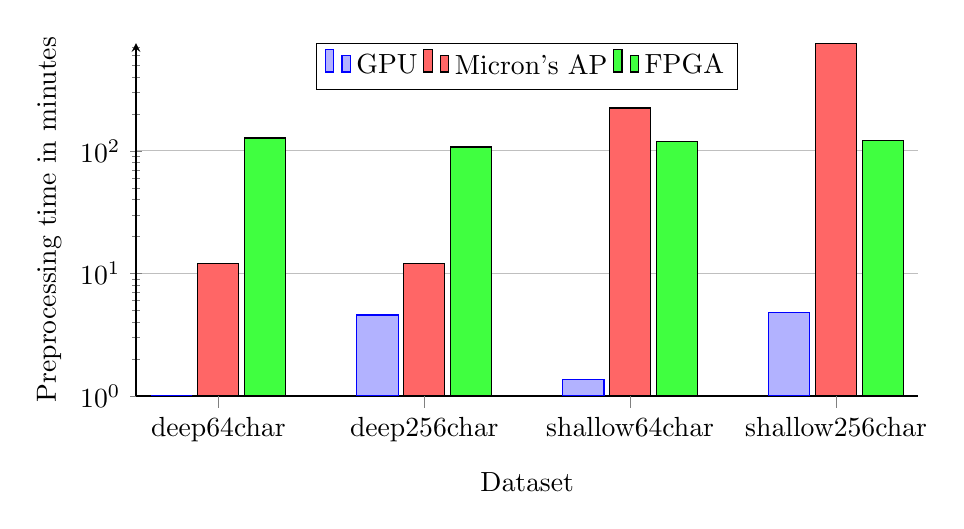
\begin{tikzpicture}
    \begin{axis}[
        ylabel=Preprocessing time in minutes,
        xlabel=Dataset,
        enlargelimits={abs=0.4},
        legend style={at={(0.5,1)},
            anchor=north,legend columns=3},
        ybar,
        bar width=0.2, % Adjust the width as needed
        xtick=\empty, % Remove numbers on the x-axis
        width=0.95 \textwidth,
        height=0.5 \textwidth,
        extra x ticks={1, 2, 3, 4}, % Add extra ticks at positions 1, 2, and 3
        extra x tick labels={deep64char, deep256char, shallow64char, shallow256char}, % Label the extra ticks
        % remove just frame, not ticks
        axis x line*=bottom,
        axis y line=left,
        ymajorgrids=true,
        ymode=log, % Set Y-axis to log scale
      ]
      \addplot
      coordinates {
          (1, 1)
          (2, 4.583333333)
          (3, 1.366666667)
          (4, 4.766666667)
        };
      \addplot[
        fill=red!60, % Set a custom color for this bar
      ]
      coordinates {
          (1, 12)
          (2, 12)
          (3, 224)
          (4, 757)
        };
      \addplot[
        fill=green!75, % Set a custom color for this bar
      ]
      coordinates {
          (1, 127.5)
          (2, 107.6)
          (3, 120.2)
          (4, 122)
        };
      \legend{GPU, Micron's AP, FPGA}
    \end{axis}
  \end{tikzpicture}
  \caption{Preprocessing time, part of figure 5 from \cite{Nourian:DemystifyingFSA}}
  \label{preprocessing:DemystifyingFSA}
\end{figure}
\subsection{Papers on speeding up FSA processing on GPUs} \label{speeding up FSA processing on GPUs}
\textit{"On-the-Fly Principled Speculation for FSM Parallelization"}\cite{zhao2015fly}, published in 2015, researched speculative execution of finite state machines. Their research was focused on DFAs. They have employed techniques to accelerate DFA executions, which have subsequently been utilised to increase GPU acceleration of DFAs.

The paper \textit{"Scaling Out Speculative Execution of Finite State Machines with Parallel Merge"} \cite{Xia:FSA-scaling}, published in 2020, develops optimisation techniques to improve the performance of DFAs execution on GPUs by extending existing work on speculative execution of FSMs and adapting it to GPU design. Their findings demonstrate significant enhancements on a scale ranging from tens to hundreds, but although it works with regular expressions, this approach has not been tested on any real dataset to verify its effectiveness in a real-world environment.

The latest paper on the execution of DFAs \textit{"GSpecPal: Speculation-Centric Finite State Machine Parallelization on GPUs"}\cite{wang2022gspecpal}, published in 2022, have addressed the existing bottlenecks, achieving an average speedup of 7.2x.

\textit{"Why GPUs are Slow at Executing NFAs and How to Make Them Faster"} \cite{Liu:WhyGPUSlowNFA}, published in 2020, improves the implementation of NFAs. The authors conducted measurements on the NVIDIA Quadro P6000 GPU\footnote{} and demonstrated more than a 25 times speedup in several applications, outperforming the AP chip in some real-world datasets, such as snort or YARA. However, it should be noted that their approach has limitations and is most effective in applications with a large number of states and is not usable with large NFA's that may occur.

The most recent research on NFAs, \textit{"Asynchronous Automata Processing on GPUs"}\cite{Liu:Asynchronous} from 2023, improved upon previous work and achieved a system that achieves a speedup of 2-50 times.

\subsection{OpenCL and CUDA implementations} \label{OpenCL and CUDA implementations}
All the studies, except for \cite{rosciszewski2014regular} which utilized OpenCL, employed CUDA for implementing their approaches. Although the research by \cite{Fang:Comparison-cuda-opencl} suggests that there is no significant difference in performance, writing optimal code appears more convenient in CUDA.

\subsection{Heteregeneous computing} \label{Heteregeneous computing}
Although research has been conducted on combining multiple accelerator platforms \cite{kobayashi2019gpu}, no work has been undertaken to utilize this method for accelerating regular expressions.

\section{Results} \label{Results}
Our analysis of the literature has demonstrated that the GPU is a viable platform for accelerating regular expressions. However, the GPU is not a universal solution and its use depends on the problem being addressed.
\subsection{Finite Automata} \label{Finite Automata:Results}
The study \cite{Becchi:regex_large_dataset} shows that DFA is the fastest solution for regular expression matching. However, a limiting factor can be the size of the DFA, especially on large datasets with multiple states, which can exceed the GPU's memory capacity. This can be alleviated by using a compressed DFA, which is slower than the uncompressed version, but faster than Non-Deterministic Finite Automata (NFA). Numerous studies have been undertaken to enhance the performance of DFA on GPU, with reference to \cite{zhao2015fly,Xia:FSA-scaling,wang2022gspecpal}. The state of the art solution \cite{wang2022gspecpal} should offer the fastest speed for some applications, but this solution has not been tested against current FPGA or AP solutions and is not known preprocessing time.

NFA has a smaller size and a much faster preprocessing time compared to DFA, although it is slower in operation, as stated in \cite{Nourian:DemystifyingFSA}. Since the time of measuring in \cite{Becchi:regex_large_dataset}, several studies \cite{Liu:WhyGPUSlowNFA,Liu:Asynchronous} have been carried out to boost NFA performance on GPUs. The latest solution \cite{Liu:Asynchronous} provides a speedup over AP chip in some real-life datasets.

No current study has yet offered data on when it is optimal to use DFA or NFA.

\subsection{Other platforms} \label{Other platforms:Results}
The research paper \cite{Nourian:DemystifyingFSA} demonstrates that for regular expression matching, FPGA and AP produce faster results compared to GPU. However, current state-of-the-art GPU solutions offer speeds that are comparable to FPGA and AP, while having significantly faster preprocessing time, as illustrated in Figure \ref{preprocessing:DemystifyingFSA}. While FPGA and AP remain superior solutions for datasets that are static and for businesses that can afford specialized solutions, GPUs are present in most devices and can be utilized for a multitude of tasks.

Currently, no studies have been conducted on the combination of multiple accelerator platforms for the acceleration of regular expressions. However, prior research has examined the potential of integrating multiple accelerator platforms \cite{kobayashi2019gpu}. It is our belief that such an approach could be utilised to accelerate regular expressions, but further research is required.

\subsection{OpenCL and CUDA implementations} \label{OpenCL and CUDA implementations:Results}
All the aforementioned studies, with the exception of \cite{rosciszewski2014regular} which used OpenCL, used CUDA to implement their approaches. According to research by \cite{Fang:Comparison-cuda-opencl}, there is no significant difference in performance, although writing optimal code in CUDA seems to be more convenient, but further research is needed.
However, using the CUDA implementation limits the ability to run the code on anything other than Nvidia GPUs.

\section{Discussion and Future work} \label{Discussion and Future work}
Our analysis couldn't provide definitive answers to the question of when to use GPU acceleration of regular expressions. Even though there have been work done on optimizing the performance of regular expressions on GPUs, there is still blank space regarding it's use in real-life applications. The current state of the art solutions provide theoreticly comparable performance to FPGA and AP, but the lack of real-life data makes it difficult to determine the optimal use case for GPUs and whether it is worth the effort to implement GPU acceleration. The lack of current research show that the topic is not currently a priority for researchers, most probably due to the fact that the current solutions are sufficient for most use cases. However, there are still some areas that could be explored.

CUDA have been the most used platform in the research, but there is a lack of research on the use of OpenCL. Usage of OpenCL would allow the code to be run on a wider range of GPUs, but it is not known whether the performance or ease of implementation would be comparable to CUDA.
Another area that could be explored is the combination of multiple accelerator platforms. The research shows that it is possible to combine multiple accelerator platforms, but it not known whether it would be beneficial for same use cases.

\section{Conclusions} \label{Conclusions}
Our study of the acceleration of regular expressions demonstrates that the GPU shows potential as a viable platform, depending on specific use cases and computational requirements. Deterministic Finite Automata (DFA) are able to perform at high speeds, although they encounter difficulties when processing large datasets due to their size. Non-Deterministic Finite Automata (NFA) present a feasible alternative since they are smaller in size and have a faster pre-processing, but the optimal circumstances for using either DFA or NFA remain unclear.

Field-Programmable Gate Arrays (FPGA) and Application Processors (AP) are superior to GPUs in terms of regular expression matching speed. Nevertheless, GPUs currently compete with FPGA and AP speeds with notably expedited preprocessing.

The possibility of combining multiple accelerator platforms with GPUs for regular expression acceleration, including an OpenCL comparison with CUDA, remains unexplored and warrants further investigation.

\bibliography{zdroje}
\bibliographystyle{abbrv}
\end{document}
